%%%%%%%%%%%%%%%%%%%%%%%%%%%%%%%%%%%%%%%%%%%%%%%%%%%%%%%%%%%%%%%%%%%%%%%%%%
%%%%%%%%%%%%%%%%%%%%%%%%%%%%%%%%%%%%%%%%%%%%%%%%%%%%%%%%%%%%%%%%%%%%%%%%%%
\clearpage{}
\section{Photon reconstruction and fake rate}
\label{sec:photon}
% ---- ---- ---- ---- ---- ---- ---- ---- ---- ---- ---- ---- ---- ---- ----
Photon candidates are reconstructed as SuperClusters in the ECAL with 
$E_{T} > 30 GeV $in the feducial Barrel region, defined by $|\eta|<1.4442$. 
They are required to satisfy 2012 tight cut-based selection 
\cite{pho2012IDcut}, which provides $70\%$ signal selection efficiency:

\begin{itemize}
\item Single tower H/E $<$ 0.05 
\item $0.001 < \sigma_{i\eta i\eta}<0.011$ 
\item PF charged hadron isolation $<$ 0.7, whith charged hadrons originated from the hard interaction primary vertex.
\item pile-up corrected PF neutral hadron isolation $< 0.4 + 0.04*P_{T}^{\gamma}$ 
\item pile-up corrected PF photon isolation $<0.5 + 0.005*P_{T}^{\gamma}$
\item Conversion safe electron veto

\end{itemize}

Isolation is performed for a cone of radius 0.3. Pile-up corrected PF isolation 
is calculated using effective area corrections. The photon candidates are
also required to be separated from the lepton by at least $0.5$ in 
$\eta-\phi$ space, which highly reduces the contribution from FSR to the 
observed photon rate. The same separation requirements are imposed between 
the photon candidates and the jets.

\subsection{Data/MC Efficiency Scale Factors}

We used photon efficiency scale factors for 2012(A+B+C+D) and tight 
photon selection described ~\cite{HtoZA-AN-13-038}, which is Egamma POG 
approved. The scale factors do not include electron veto selection and 
are listed in Table~\ref{tab:photon_eff}. The scale factors for electron 
veto selection are $0.9958 \pm 0.0043 (E_{T}=[30,40] GeV)$ and 
$0.9999 \pm 0.0067 (E_{T}>40 GeV).$ 

\begin{table}[htb]
\centering
    \begin{tabular}{|l|l|c|}
      \hline
      SC $\eta$                     & $E_{T}$ (GeV) & Scale factor  \\ \hline
      \multirow{4}{*}{0.0 - 0.8}    & 30-40         & $0.9711 \pm 0.0020$     \\
                                    & 40-50         & $0.9778 \pm 0.0024$     \\
                                    & 50-Inf        & $0.9718 \pm 0.0014$     \\ \hline
      \multirow{4}{*}{0.8 - 1.4442} & 30-40         & $0.9823 \pm 0.0052$     \\
                                    & 40-50         & $0.9805 \pm 0.0024$     \\
                                    & 50-Inf        & $0.9768 \pm 0.0016$     \\ \hline
    \end{tabular}
  \caption{2012 tight photon ID data/MC efficiency scale factors for given photon $p_{T}$ and $\eta$ ~\cite{HtoZA-AN-13-038}.  }
  \label{tab:photon_eff}
\end{table}

\subsection{2012 Photon ID Fake Rate}

The largest background arises from the $W\gamma$+jets process, while the 
second important contribution comes from jets or electrons misidentified as
a photon. Electrons could be identified as photons due to small track 
reconstruction inefficiency of the detector. This contribution is relevant 
to the electron channel, when an electron or positron from 
$Z\rightarrow ee$ passes the photon identification criteria; therefore, to 
reduce this background, we impose a 
$|M_{Z}-M_{e\gamma}| > \textnormal{10 GeV}$ cut. Events with jets 
misidentified as photons can not be tagged with a simple kinematic 
requirement, because it resembles the topology of the events with true
photons. The adopted approach is to build the expected rate based on the 
ratio method \cite{VgammaPAS}. The method uses a category of 
jets(photon-like jets), which resembles the electromagnetic objects in the 
ECAL, but fail either the isolation or $\sigma_{i\eta i\eta}$ requirement. 
Through simple algebraic conversion it can be made into the photon fake 
rate, or number of fake photon candidates divided by the total number of all
photon candidates. We perform a very similar fake rate estimation using our
full 2012 single lepton dataset and assign a $p_{T}$-dependent systematic
uncertainty on the fake rate estimation. 

Similar to the Egamma method, for our fake rate estimation we use the 
full 2012 dataset with single lepton triggers (that we use in our 
analysis) to form a signal and background template that will be 
normalized to each other's sideband. This is to say that we estimate our 
data-driven fake rate by: filling the signal distribution in 
$\sigma_{I\eta I\eta}$ with 2012 tight photons; filling the background 
distribution in $\sigma_{I\eta I\eta}$ with 2012 photon candidates that fail 
the tight cut in particle flow charged and/or neutral isolation, as well 
as possibly failing the tight $\sigma_{I\eta I\eta}$ cut; and normalizing the
background distribution's $\sigma_{I\eta I\eta}$ sideband (
$\sigma_{I\eta I\eta} >$ 0.011) to the sideband of the signal's distribution.
In order to preserve the sidebands of the signal and background 
$\sigma_{I\eta I\eta}$ distributions, we remove the $\sigma_{I\eta I\eta}$ cut in
the 2012 tight photon ID. We normalize the background's sideband to the 
signal sideband because we call any photon candidates that fail the tight
$\sigma_{I\eta I\eta}$ a fake photon, or photon-like jet; therefore, any
contribution in the signal distribution above $\sigma_{I\eta I\eta} >$ 0.011
comes from the background, or fake photons. 
Figure~\ref{fig:normalizeFake} demonstrates how the backgrounds' 
sidebands have been normalized to the signals' sidebands for each photon
$p_{T}$ bin.

\begin{figure}[]
  \begin{center}
    \subfigure[]{
    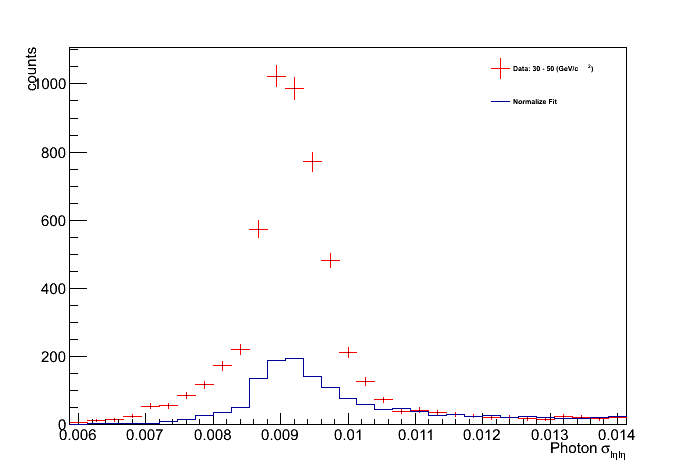
\includegraphics[width=0.33\textwidth]{figs/normalize_fit_30_to_50.png}
  }
    \subfigure[]{
    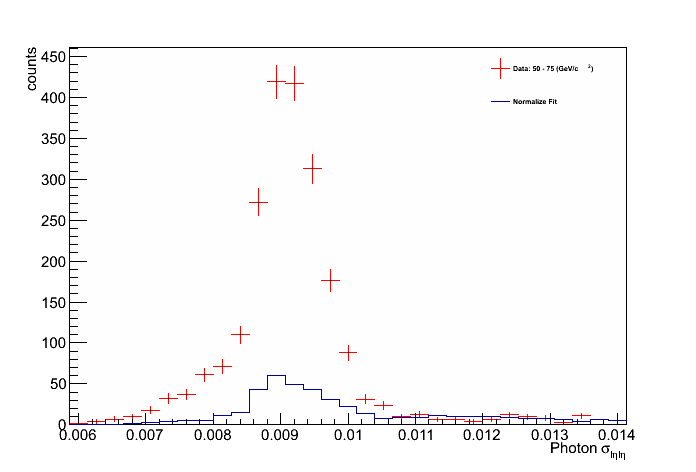
\includegraphics[width=0.33\textwidth]{figs/normalize_fit_50_to_75.png}
  }
    \subfigure[]{
    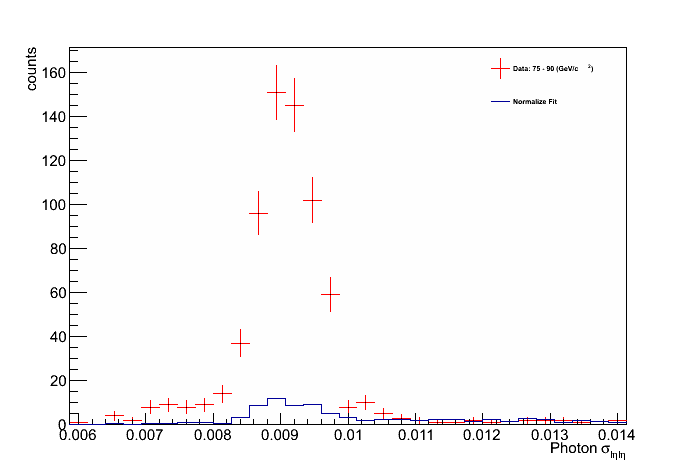
\includegraphics[width=0.33\textwidth]{figs/normalize_fit_75_to_90.png}
  }\\
    \subfigure[]{
    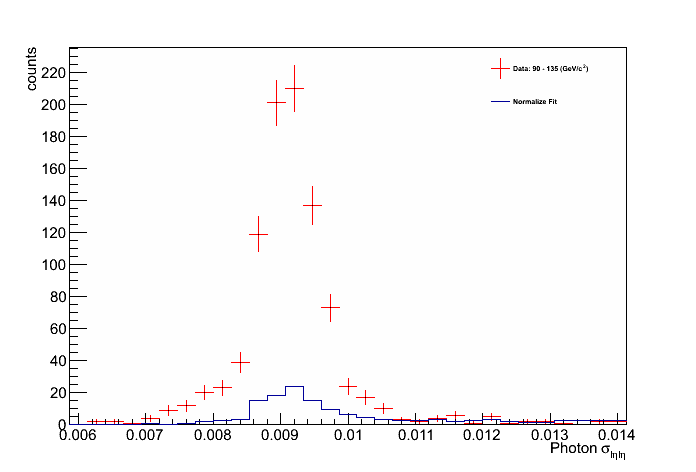
\includegraphics[width=0.33\textwidth]{figs/normalize_fit_90_to_135.png}
  }
    \subfigure[]{
    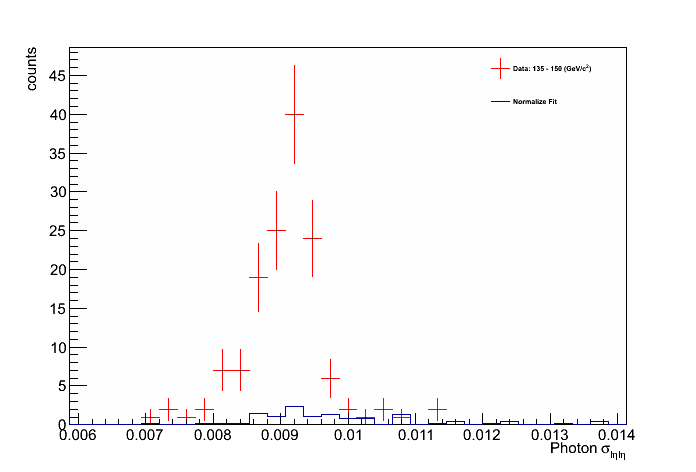
\includegraphics[width=0.33\textwidth]{figs/normalize_fit_135_to_150.png}
  }
    \subfigure[]{
    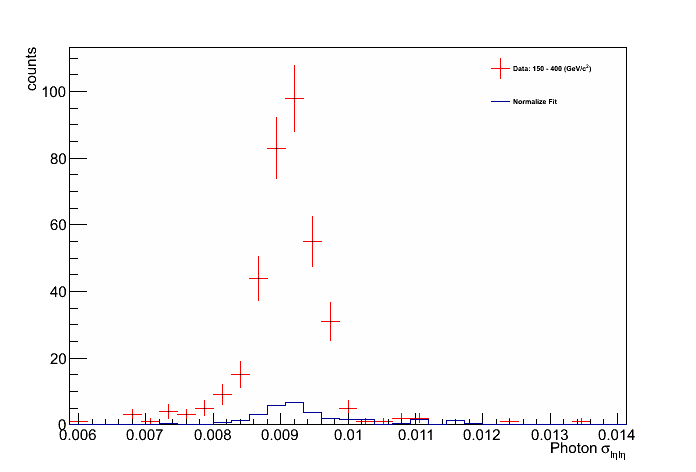
\includegraphics[width=0.33\textwidth]{figs/normalize_fit_150_to_400.png}
  }
    \caption{Signal and background distributions in $\sigma_{I\eta I\eta}$ used to estimate the WW$\gamma$ photon-like jet, or fake photon, rate. Red points are from 2012 tight photons, while blue points are 2012 photon candidates that fail tight PF charged and/or neutral isolation. The background's sideband (above 0.011) is normalized to the signal. Photon $p_{T}$: (a) 30-50 GeV/c, (b) 50-75 GeV/c, (c) 75-90 GeV/c, (d) 90-135 GeV/c, (e) 135-150 GeV/c, (f) 150-400 GeV/c}
    \label{fig:normalizeFake}
  \end{center}
\end{figure}

With the two distributions' sidebands normalized in each photon $p_{T}$ 
bin, we estimate the fake-photon contamination within the signal 
distribution by integrating the background below $\sigma_{I\eta I\eta}$ of 
0.011. Thus, with the number of background, or photon-like jets, and the 
number of 2012 tight photons below this cut, we can estimate our 
analysis's $p_{T}$-dependent photon fake rate, as shown in 
Table~\ref{tab:WWAfakerate}. We only estimate the rate for barrel photons
currently.

\begin{table}[bthp]
\begin{center}
{\footnotesize
\begin{tabular}{|c|c|}
\hline
Photon $p_{T}$, & Fraction of events with jets,\\
GeV & passing tight photon ID\\

\hline
30-50    &  0.229\\
50-75    &  0.156\\
75-90    &  0.091\\
90-135   &  0.122\\
135-150  &  0.080\\
150-400  &  0.077\\
\hline
\end{tabular}
\caption[.]{\label{tab:WWAfakerate}
WV$\gamma$ Fake rate from q-jets and tight 2012 photon ID.}}
\end{center}
\end{table}

In order to estimate the systematic uncertainty in the photon fake rate,
two separate contributions are considered - the effect of biasing the
fake photon template, and the statistical uncertainty in the bias
measurement. The known bias is that the fake photon template is
constructed using inverted PF isolation in the 2012 photon tight selection
ID, where it is assumed that all photon candidates filling this template
are in fact jets faking a photon.  

To test this bias, a MC sample
containing jets misidentified as photons is used (such as W+jets MC), along with its
generator information for all jets and photons, to construct the truth
and estimate templates. The muon channel of the MC is used for this study
in order to remove the photon-faking electron contribution.  The generator information 
is used to remove all ISR/FSR
photons from the pool of 2012 tight photon candidates in the MC, leaving only
those photon candidates that must be jets misidentified as photons - these will
fill the truth template. The estimate template is filled using the aforementioned
inverted isolation procedure for all photon candidates in the MC. The two
templates are compared using the same prescription described for the data-driven
fake rate estimate of the prompt and fake photon templates; however, due to low
statistics in MC after removing all prompt photons, the entire photon $p_{T}$ range
is used to fill one truth template and one estimate template. Any deviation from a
100\% match between the true and estimate templates is considered to be the
measurement of the bias. The bias is measured to be -6\% $\pm$ 11\%, or that the 
truth and estimate templates are in 94\% agreement. The uncertainty in this measurement
is included in the overall systematic uncertainty in the fake rate.

The photon $p_{T}$-dependent statistical uncertainty is estimated using toy MCs -
histograms filled with similar statistics as those of the data-driven fake photon
templates, using a random filler. The toy MC histograms
are then treated as the new fake photon templates, while still using the data-driven
prompt photon templates, and the fake photon rate is
remeasured. The RMS of the measurement of the fake rate for all toy MCs is made
the statisticly-driven uncertainty in the fake rate systematic uncertainty. Table~\ref{tab:fakerate_unc}
contains the photon $p_{T}$-dependent statistical uncertainties in the fake rate, where
the last two photon $p_{T}$ bins mentioned earlier (135-150 GeV and 150-400 GeV) have
been combined due to low statistics. The measured systematic and statistical uncertainties
are combined to make the photon $p_{T}$-dependent systematic uncertainties listed in 
Table~\ref{tab:sys_unc}.

\begin{table}[htb]
\centering
    \begin{tabular}{|c|c|c|c|c|}
      \hline
      $E_{T}$ (GeV) & Fake Rate & Stat. Unc. & Stat. Unc. (\%) & Bias Stat. Unc. (\%)  \\
      \hline
      30-50         & 0.229     & 0.0128     & 5.6             & 11 \\
      50-75         & 0.156     & 0.0147     & 9.4             & 11 \\
      75-90         & 0.091     & 0.0184     & 20              & 11 \\
      90-135        & 0.122     & 0.0230     & 19              & 11 \\
      135-400       & 0.078     & 0.0287     & 37              & 11 \\
      \hline
    \end{tabular}
  \caption{2012 tight photon ID data-driven photon-faking jet rate plus uncertainties for given photon $p_{T}$.  }
  \label{tab:fakerate_unc}
\end{table}

When selecting fake-photon events from our data in order to complete our
analysis for aQGC, the photon-like jet selection satisfies 2012 loose 
cut-based selection \cite{pho2012IDcut}, while it is also required to 
fulfill at least one of following:

\begin{itemize}
\item $\sigma_{i\eta i\eta}>0.012$
\item PF charged hadron isolation $> 4.0 $
\item pile-up corrected PF neutral hadron isolation $> 4.5 +0.04*P_{T}^{\gamma}$
\item pile-up corrected PF photon isolation $>4.5 + 0.005*P_{T}^{\gamma}$

\end{itemize}

These events are then weighted according to the fake ratio derived from
our fake rate.

%We also restrict our analysis to barrel photons by imposing a $|{\eta}| < \textnormal{1.4442}$ cut.  We choose to ignore events with photons detected in the endcaps because the rate of falsely identified photons, or fake photons, as well as the systematics for estimating such a rate, increases outside of the barrel region.  A $p_{T}$ threshold of 30 GeV is used, also due to the fake photon rate that will be discussed - specifically because the rate is only defined down to photon $p_{T}$ of 32 GeV.  Another fake photon contribution considered is that of a Z boson decaying to two electrons, where one of the electrons gets misidentified as a photon; therefore, to reduce this background we impose a $|M_{Z}-M_{e\gamma}| > \textnormal{10 GeV}$ cut.  All selected photons are also required to be isolated from jets and leptons with an isolation cone of size 0.5 or greater.

%The Vgamma photon fake rate considered jets consisting of $\pi_{0}\textnormal{'s}$.  In order to estimate the rate of such jets being misidentified as photons, they performed a two-component template fit using 2011 A\&B photon secondary datasets and a diphoton Monte Carlo sample.  The data and Monte Carlo signal templates were created using the 2011 tight photon ID mentioned earlier, without the sigmaIetaIeta cut, while the Monte Carlo background template used all the same cuts with the exception of inverting the Track isolation cut.  The sigmaIetaIeta cut was removed from the templates in order to preserve the sidebands used in the template fit.  Since the photon fake rate is also known to be dependent on both $\eta$ and photon $p_{T}$, the templates were made for specific $\eta$ and photon $p_{T}$ ranges and compared in the final result shown in Figure~\ref{fig:fkrate}.

%The distribution shown in Figure~\ref{fig:fkrate} is the photon fake ratio, or the number of fake photon candiates divided by the number of true photon candidates, and through algebraic conversion it can be made into the photon fake rate, or number of fake photon candidates divided by the total number of all photon candidates.  In order to use this Vgamma photon fake rate in our analysis, we fit the distribution shown above with a function and applied it as a weight scale factor on the 2012 full dataset.  This means that the function estimates what fraction of the observed data events are likely to include a jet misidentified as a photon.

